\documentclass[10pt,t]{beamer} % handout
\usetheme{Heverlee}
\usepackage{animate}
\usepackage{tikz}
\usepackage{tikz-cd}
\usepackage{svg}
\usepackage{bm}
% notes
\usepackage{pgfpages}
\setbeameroption{show notes on second screen}
\setbeamertemplate{note page}{%
	\vskip 10pt
	\lineskip 5pt
	\large
	\insertnote
}
\newcommand{\vk}{\vskip 5pt}
\usepackage{mathtools}

\newcommand{\R}{\mathbb{R}}

\setbeamertemplate{theorems}[numbered] 
\newtheorem{result}{Result}

%%% QUICK OPTIONS:
% (A) Math font without serifs, enable line below to make math serif:
    \usefonttheme[onlymath]{serif}

% (B) Re-define primary colour by adjusting the RGB values
%    \definecolor{pblue}{RGB}{206,125,66}

% (C) Title page graphic (optional) --- this is not for the background image, see \usebackgroundtemplate to change that ---
    %\titlegraphic{\includegraphics[height=2.7cm]{example_figure.pdf}}

% (D) Add logo to bottom right-corner (optional)
    \logo{\includegraphics[height=0.7cm]{icosahedron-src.pdf}\hspace{12pt}\vspace{-6pt}} 

% (E) Choose one (or none) of these lines to add footline bar on all frames
    %\setbeamertemplate{footline}[infoline]  % author, title, insitute
    %\setbeamertemplate{footline}[navigation] % dots swhowing progress
    %\setbeamertemplate{footline}[navsym] % navigation symbols

% (F) Widescreen 16:9 ratio
    %\usepackage[orientation=landscape,size=custom,width=16,height=9,scale=0.45,debug]{beamerposter} 

%%% TITLE PAGE INFO:

\title{Derived Commutativity in Data Science,\\ Category Theory, and Quantum Physics}
\subtitle{Theoretical and computational aspects}
\author[ammedmar]{Anibal M. Medina-Mardones}
\institute{Max Planck Institute for Mathematics}
\date{March 2021}

\begin{document}
{
% Change image, or delete this line to remove background image
\usebackgroundtemplate{ \parbox[b][\paperheight][b]{\paperwidth}{\centering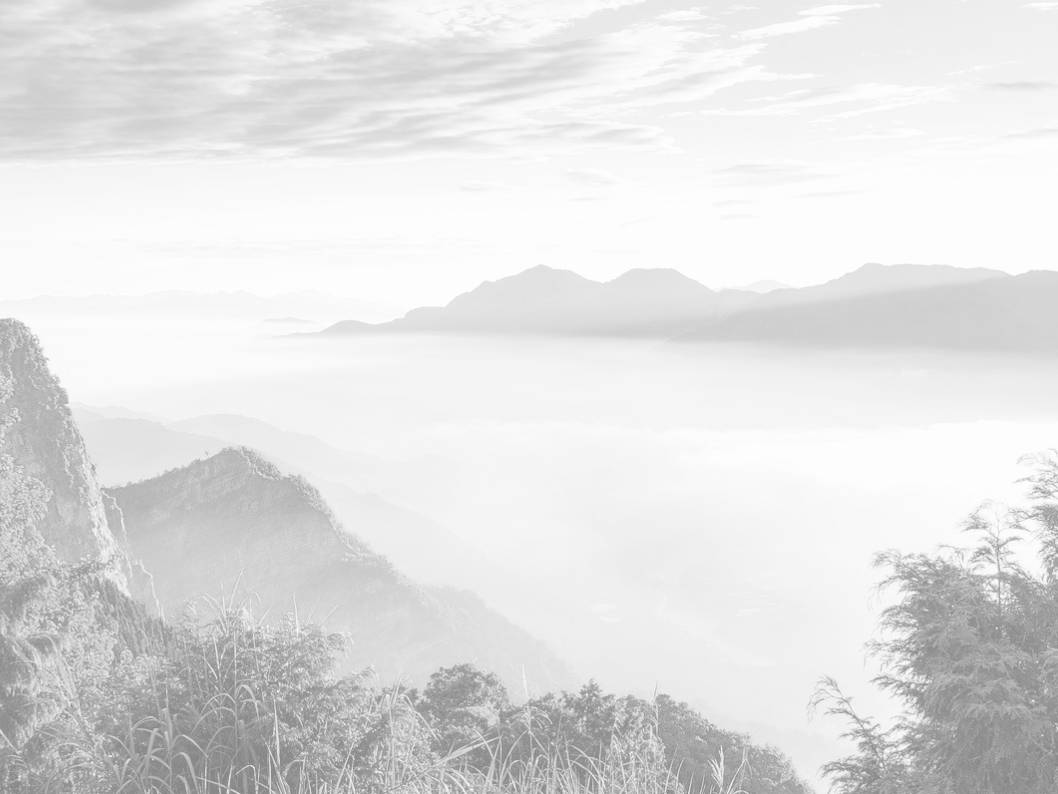
\includegraphics[width=\paperwidth]{bg_alishan.jpg}}} 
 %   abudhabi      cherry      forest      river
 %   alishan       chobe       leuven      sanfancisco
 %   blueprint     columns     library     uyuni
 %   bokeh         flowers     newyork     winter

%\setbeamercolor{background canvas}{bg=lgray}  % make background light gray

% Title page
\begin{frame}[plain, noframenumbering]
    \titlepage
    \note{Thank you, it's great to be here.}
\end{frame}
}

% Table of contents slide
\begin{frame}{Outline}
	\vskip 2mm
	\hfill{\large \parbox{.95\textwidth}{\tableofcontents[hideothersubsections]}}
	\note{The plan for today}
\end{frame}

\section{From data to topology}

\note{Let's start here}

\begin{frame}{Point clouds}
	\note{
		We can think of a point cloud of data, as obtained by sampling from a probability distribution function on $\R^n$.
		\vk
		These tend to concentrate around lower dimensional subspaces.
		\vk
		We would like to have ways to study this underlying space.
		\vk
		We can use triangulations to approximate it at different scales.
		
		Given a scale parameter $r$, we join pairs of points with an edge if their distance is less that $r$,
		
		if 3 points have pairwise distance less than $r$, then we place a triangle between them,
		
		and for 4 points, we include tethrahedra and so forth.
		\vk
		Instead of picking a scale, we can consider the entire family of approximating triangulations, and notice there is some structure here
		
		if $r$ is less than $r^\prime$, then the approximation at scale $r$ is part of that at $r^\prime$.
	}
	\begin{itemize}
		\item A data set can often be thought of as a point cloud in $\R^n$.
		
		\vskip 8pt
		
		\item Underlying probability distribution concentrated in a subspace.
		
		\vskip -5pt
		
		\begin{center}
			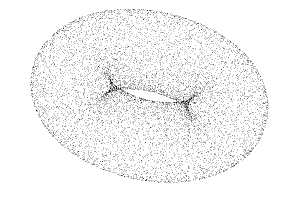
\includegraphics[scale=.3]{torus}
		\end{center}
		
		\pause 
		
		\item How to approximate and study the underlying shape?
		
		\pause
		\vskip 5pt
		
		\begin{center}
			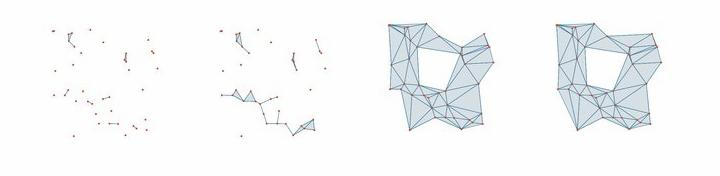
\includegraphics[scale=.4]{filtration}
		\end{center}
	
		\vskip -3pt
		
		Approximate using a multiscale construction.
	\end{itemize}
\end{frame}

\begin{frame}{Persistence homology}	
	\begin{itemize}
		\item Study through construction of invariants of the associated shapes.
		
		\pause
		
		\item Topology provides principled ways of constructing invariants.
		
		\vskip 10pt
		\begin{center}
			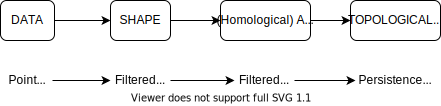
\includegraphics[scale=.5]{diagram}
		\end{center}
	
		\pause
		\item \textcolor{pblue}{Machine Learning Intuition}: The 0-dimensional part of this invariant is equivalent to hierarchical clustering.
		
		\begin{center}
			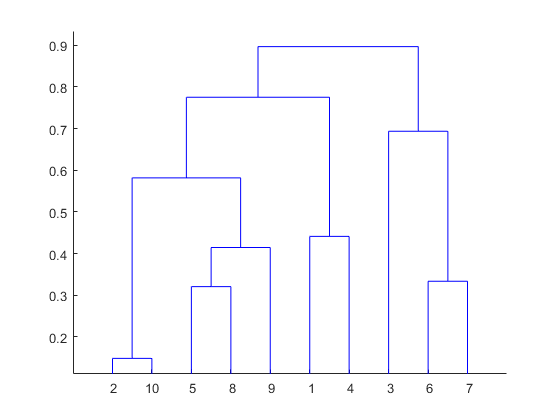
\includegraphics[scale=.2]{dendogram}
		\end{center}
	\end{itemize}	
\end{frame}

\begin{frame}{Example: Nanoporous materials}
	as
\end{frame}

\begin{frame}{Machine Learning and Topology}
	Is there a way for ML practitioners to easily incorporate persistence homology into standard pipelines?
	
	\vskip 10pt
	\pause
	
	\includegraphics[scale=.31]{giotto}	
\end{frame}

\section{Finer invariants}

\begin{frame}{Finer topological invariants}
	\newcommand*{\xMin}{0}%
	\newcommand*{\xMax}{4}%
	\newcommand*{\yMin}{0}%
	\newcommand*{\yMax}{4}%
	\begin{center}
	\begin{tikzpicture}[scale=.6]
	\draw[-{Latex[length=2mm]}] (-.5,\yMin)--(-.5,\yMax);
	\draw[-{Latex[length=2mm]}] (-.5,\yMin)--(-.5,\yMax-.5);
	\draw[-{Latex[length=2mm]}] (4.5,\yMin)--(4.5,\yMax);
	\draw[-{Latex[length=2mm]}] (4.5,\yMin)--(4.5,\yMax-.5);
	
	\draw[-{Latex[length=2mm]}] (\xMin, -.5)--(\xMax, -.5);
	\draw[-{Latex[length=2mm]}] (\xMin, 4.5)--(\xMax, 4.5);
	
	\draw (0,0)--(0,4)--(4,4)--(4,0)--(0,0);
	
	\node at (2,-1.2){$T$};
	\end{tikzpicture}
	\hspace*{2cm}
	\begin{tikzpicture}[scale=.6]
	\draw[-{Latex[length=2mm]}] (-.5,\yMin)--(-.5,\yMax);
	\draw[-{Latex[length=2mm]}] (-.5,\yMin)--(-.5,\yMax-.5);
	\draw[-{Latex[length=2mm]}] (4.5,\yMax)--(4.5,\yMin);
	\draw[-{Latex[length=2mm]}] (4.5,\yMax)--(4.5,\yMin+.5);
	
	\draw[-{Latex[length=2mm]}] (\xMin, -.5)--(\xMax, -.5);
	\draw[-{Latex[length=2mm]}] (\xMin, 4.5)--(\xMax, 4.5);
	
	\draw (0,0)--(0,4)--(4,4)--(4,0)--(0,0);
	
	\node at (2,-1.2){$K$};
	\end{tikzpicture}
	\end{center}
\end{frame}

\begin{frame}{Finer topological invariants}
	\newcommand*{\xMin}{0}%
	\newcommand*{\xMax}{4}%
	\newcommand*{\yMin}{0}%
	\newcommand*{\yMax}{4}%
	
	\begin{center}
	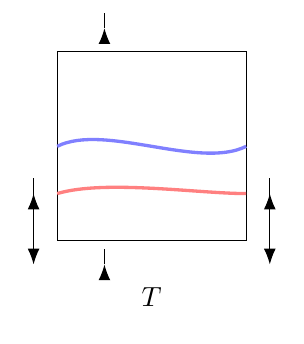
\begin{tikzpicture}[scale=.6]
	\draw[-{Latex[length=2mm]}] (-.5,\yMin)--(-.5,\yMax);
	\draw[-{Latex[length=2mm]}] (-.5,\yMin)--(-.5,\yMax-.5);
	\draw[-{Latex[length=2mm]}] (4.5,\yMin)--(4.5,\yMax);
	\draw[-{Latex[length=2mm]}] (4.5,\yMin)--(4.5,\yMax-.5);
	
	\draw[-{Latex[length=2mm]}] (\xMin, -.5)--(\xMax, -.5);
	\draw[-{Latex[length=2mm]}] (\xMin, 4.5)--(\xMax, 4.5);
	
	\draw (0,0)--(0,4)--(4,4)--(4,0)--(0,0);
	
	\draw[color=blue!50, very thick] (0,2) .. controls (1,2.5) and (3,1.5) .. (4,2);
	\draw[color=red!50, very thick] (0,1) .. controls (1,1.3) and (3,1) .. (4,1);
	
	\node at (2,-1.2){$T$};
	\end{tikzpicture}
	\hspace*{2cm}
	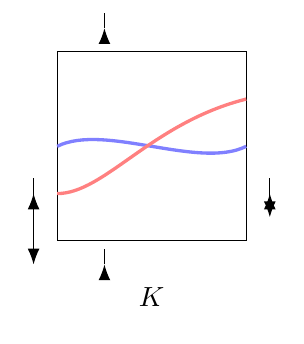
\begin{tikzpicture}[scale=.6]
	\draw[-{Latex[length=2mm]}] (-.5,\yMin)--(-.5,\yMax);
	\draw[-{Latex[length=2mm]}] (-.5,\yMin)--(-.5,\yMax-.5);
	\draw[-{Latex[length=2mm]}] (4.5,\yMax)--(4.5,\yMin);
	\draw[-{Latex[length=2mm]}] (4.5,\yMax)--(4.5,\yMin+.5);
	
	\draw[-{Latex[length=2mm]}] (\xMin, -.5)--(\xMax, -.5);
	\draw[-{Latex[length=2mm]}] (\xMin, 4.5)--(\xMax, 4.5);
	
	\draw (0,0)--(0,4)--(4,4)--(4,0)--(0,0);
	
	\draw[color=blue!50, very thick] (0,2) .. controls (1,2.5) and (3,1.5) .. (4,2);
	\draw[color=red!50, very thick] (0,1) .. controls (1,1) and (2,2.5) .. (4,3);
	
	\node at (2,-1.2){$K$};
	\end{tikzpicture}
	\end{center}
	
	Although $H^\bullet(T, \mathbb F_2) \cong H^\bullet(K, \mathbb F_2)$ as graded vector spaces $T \not\cong K$.
	
	\vskip 5pt
	\pause
	There is more algebraic structure that distinguishes them
	\begin{align*}
	\smallsmile & \colon H^\bullet \otimes H^\bullet \to H^\bullet && \text{(commutative ring structure)},\\
	Sq^k & \colon H^\bullet \to H^\bullet && \text{(module over Steenrod algebra)}.
	\end{align*}
\end{frame}

\begin{frame}[c]{Alexander-Whitney \& Steenrod}
	\vskip -9pt
	In the 1930's Alexander, Kolmogorov, \v{C}ech and Whitney defined
	\begin{equation*}
	\smallsmile \colon H^\bullet \otimes H^\bullet
	\end{equation*}
	\vskip -9pt
	via
	\vskip -9pt
	\begin{equation*}
	\smallsmile_0 \colon C^\bullet \otimes C^\bullet \to C^\bullet.
	\end{equation*}
	
	\vskip 5pt
	\pause
	
	In the late 1940's Steenrod homotopically corrected the lack of commutativity of $\smallsmile_0$ explicitly introducing
	\begin{equation*}
	\smallsmile_i \colon C^\bullet \otimes C^\bullet \to C^\bullet,
	\end{equation*}
	and used them to define
	\begin{equation*}
	Sq^k \colon H^\bullet \to H^\bullet.
	\end{equation*}
	Their importance in stable homotopy theory is hard to overstate.
	
	\vskip 15pt
	\pause
	
	 \textcolor{pblue}{What about the $\smallsmile_i$-products?}
\end{frame}

\begin{frame}[c]{Cup-$i$ products}
	
	\vskip -10pt
	\begin{result}[Medina-Mardones]
		Just like the $Sq^k$ can be axiomatized, the $\smallsmile_i$ can be as well, and\\ all known constructions satisfy these axioms.
	\end{result}

	\pause
	\vskip 10pt
	
	\begin{result}[M-M]
		New description of the $\smallsmile_i$-products leading to \\
		incorporation of $Sq^k$ into persistence homology, and \\
		high performance implementation under development (giotto-tda's team).
	\end{result}
	
	\pause
	\vskip 10pt
	
	\begin{result}[M-M]
		The $\smallsmile_i$-products determine another fundamental construction: the nerve of strict infinity categories.
	\end{result}
\end{frame}

\section{Even finer invariants}

\begin{frame}{Secondary operations}
	The $Sq^k$ invariants are referred to as primary operations.
	
	\vskip 10pt
	
	Their relations lead to secondary operations.
	
	\pause
	
	\begin{align*}
	& Sq^k(\alpha \smallsmile \beta) = \sum_{i+j=k} Sq^i(\alpha) \smallsmile Sq^j(\beta), &&
	\text{(Cartan relation)} \\	
	& Sq^i Sq^j(\alpha) = \sum_{k=0}^{\lfloor i/2 \rfloor} {j-k-1 \choose i-2k} Sq^{i+j-k} Sq^k(\alpha) &&
	\text{(Adem relation)}
	\end{align*}
	
	\vskip 5pt
	\textcolor{pblue}{Can these by effectively computed?}
	\vskip 10pt
	
	\pause
	
	More explicitly, since these can be interpreted as relations of $\smallsmile_i$-products, can we find operations enforcing them at the cochain level?
\end{frame}

\begin{frame}[c]{Relations}
	
	\begin{result}[M-M]
		Effective construction of Cartan coboundaries.
	\end{result}

	Work motivated by physicist A. Kapustin (Caltech) and R. Thorngren (Harvard). They used my formula in lattice field theory.
	
	\begin{center}
		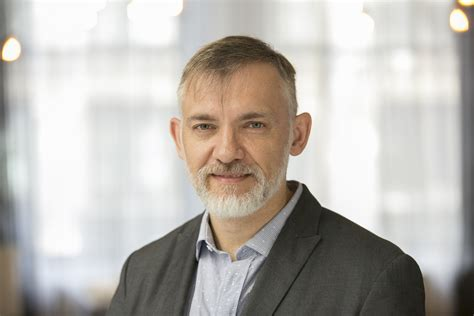
\includegraphics[scale=.13]{kapustin}
		\hspace*{1cm}
		
\includegraphics[scale=.21]{thorngren}
	\end{center}
	
	\pause
%	\vskip 20pt
	
	\begin{result}
		Effective construction of Adem coboundaries.
	\end{result}

	The above is joint with G. Brumfiel (Stanford) and J. Morgan (Columbia).
	
	\begin{center}
		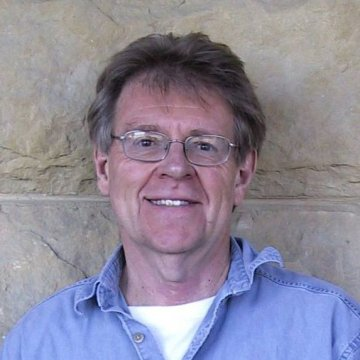
\includegraphics[scale=.21]{brumfiel}
		\hspace*{1cm}
		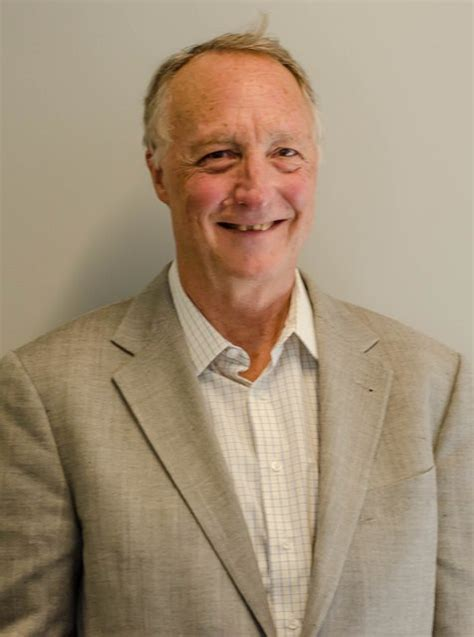
\includegraphics[scale=.09]{morgan}
	\end{center}
	
\end{frame}

\begin{frame}{Odd primes}
	
	So far we have focused on $\mathbb{F}_2$ coefficients.
	
	\vskip 5pt
	
	
	What about odd primes?
	
	\pause
	\vskip 5pt
	
	
	\begin{result}
		Effective construction of a generalization of the $\smallsmile_i$-products to coefficients in $\mathbb F_p$ for any prime $p$.
	\end{result}
	joint with R. Kaufmann (Purdue).
	
	\begin{center}
		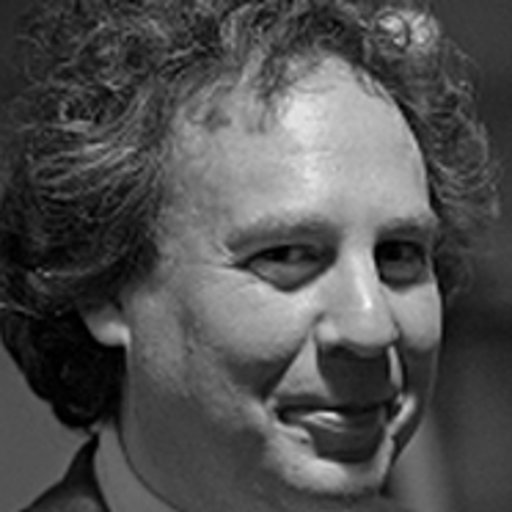
\includegraphics[scale=.1]{kaufmann}
	\end{center}
	
	\pause
	\vskip 9pt
	
	\textcolor{pblue}{What made these advances possible?}
	
\end{frame}

\section{The operadic viewpoint}

\begin{frame}{Operads}
	
	\vskip -5 pt
	
	\textcolor{pblue}{Analogy}:	abstract groups are to group representations as	\\
	Operads are to algebras (commutative, or Lie, or associative, or $\dots$)	
	
	\vskip 5 pt
	\pause
	
	Now a days we understand that the ``derived" version of a commutative algebra is an algebra over an $E_\infty$-operad. \note{This is a notion defined only up-to--homotopy, like the classifying space of principal bundles.}
	
	\vskip 5 pt
	\pause
	
	There are effective models due to McClure-Smith and Berger-Fresse.
	
	\begin{result}[M-M]
		A computer algebra system on Python for the study of these operads and their algebras. (Right place to implement some of the earlier results).
	\end{result}
	
	\vskip 5 pt
	\pause
	
	More theoretically,
	
	\begin{result}[M-M]
		Although no finitely presented $E_\infty$-operad can exist, I constructed a finitely presented prop $\mathcal M$ whose associated operad is $E_\infty$. Furthermore, \\
		this operad is cofibrant and compatible with previous models.		
	\end{result}
\end{frame}

\section{Back to data (time permitting)}

\begin{frame}{Graph Laplacian}
	A powerful tool to study weighted networks. 
	
	\vskip 5pt
	\pause
	
	\begin{center}
		\includegraphics[scale=.5]{graph}
	\end{center}
	
	\vskip -5pt
	
	\begin{equation*}
	\resizebox{8.5cm}{!}{
		$\partial =
		\begin{pmatrix*}[r]
		-1 & -1 &  0 \\
		 1 &  0 & -1 \\
		 0 &  1 &  1
		\end{pmatrix*}
		\qquad
		W =
		\begin{pmatrix*}[r]
		w_{01}& 0      & 0 \\
		0     & w_{01} & 0 \\
		0     &      0 & w_{12}
		\end{pmatrix*}
		\qquad
		\delta =
		\begin{pmatrix*}[r]
		-1 &  1 & 0 \\
		-1 &  0 & 1 \\
		 0 & -1 & 1
		\end{pmatrix*}$}
	\end{equation*}
		
	\vskip 10pt
	\pause
	
	Two types of uses:
	\begin{itemize}
		\item[] \textcolor{pblue}{Structural (eigenvalues).}	The spectrum as a feature of the graph.
		
		\pause
		
		\item[] \textcolor{pblue}{Functional (eigenvectors).} A Fourier basis for signals on the graph, \\ 
		
		\vskip 5pt
		\hspace*{5cm} \pause i.e., real numbers at every node.
	\end{itemize}

	\pause
	
	What if the signals are defined \\
	\textcolor{pblue}{\ \ \ not just on single nodes?}
\end{frame}

\begin{frame}{Information signals}
	
	Emergent phenomena in complex systems 
	
	\begin{center}
		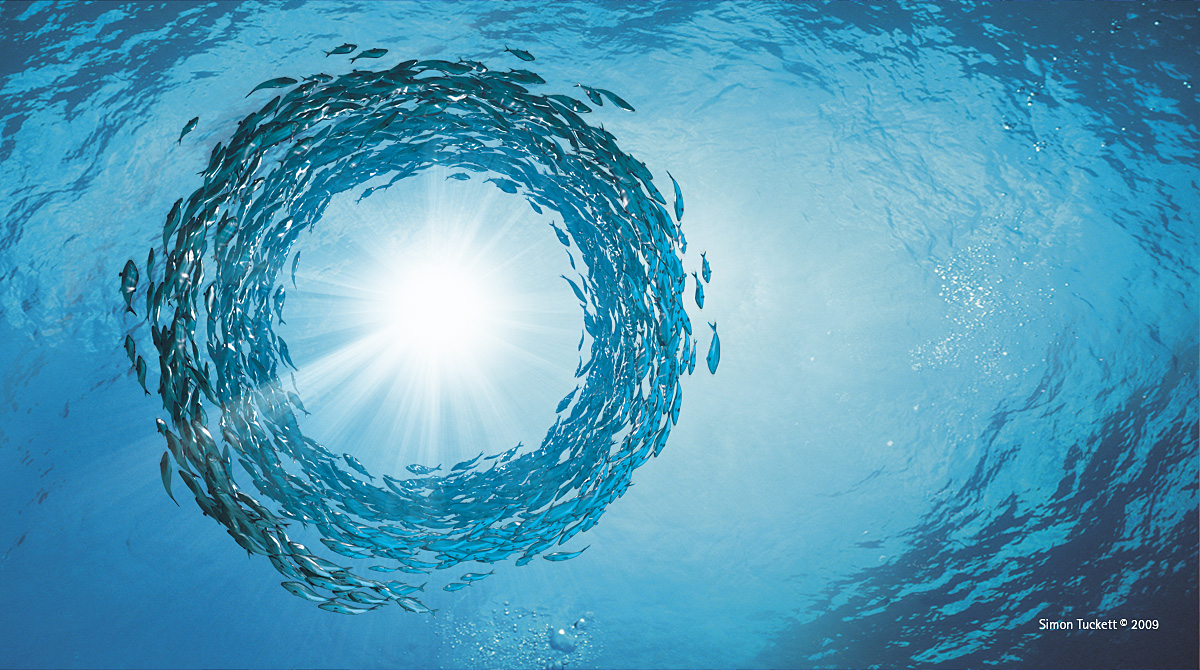
\includegraphics[scale=.15]{fishes}
	\end{center}

	\vskip 5pt
	\pause
	
	Given collection of probability distributions $X_0, \dots, X_N$, can assign to
	
	\vskip 5pt
	
	\quad Pairs: their mutual information, \\
	\quad Triples: their interaction information, and\\
	\quad $(n+1)$-element sets: higher analogues of these.
	
	\vskip 5pt
	\pause
	
	\textcolor{pblue}{Problem:} The number of subsets grows exponentially with $n$.
\end{frame}

\begin{frame}{Hyperharmonic analysis}
	
	\vskip -5pt
	
	\textcolor{pblue}{Analogy:} Need only hear a few harmonics to distinguish a guitar's from a piano's middle C.
	
	\vskip 5pt
	\pause
	
	\begin{result}
		Propose a principled method to compress high-order information signals based on Fourier analysis and combinatorial topology.
	\end{result}

	Joint with F. Rosas (Imperial College), Sebasti\'an Rodriguez (UTFS, Chile) and Rodrigo Cofr\'e (PUCV, Chile). 
	
	\vskip 5pt
	\pause
	
	\textcolor{pblue}{We use:} Eigenvectors of a discrete analogue $L_n$ of the Laplace-de Rham operator of Riemannian geometry generalizing the graph Laplacian $L_0$.
	
	\vskip 5pt
	\pause
	
	\textcolor{pblue}{Compression:} How many components we need to reconstruct the signal?
	
	\vskip 5pt
	\pause
	
	Consider a given $n$-dimensional high-order signal,
	whose coefficients on the given basis are $\bm\alpha = \{\alpha_i\}$. Assume that $\alpha_i^2 \geq \alpha^2_j$ if $i \leq j$.
	\begin{equation*}
	\text{EV}_{\alpha}(k) = \frac{ \alpha_k^2}{{\displaystyle \sum_{i} \alpha_i^2}}
	\qquad \text{ and } \qquad
	\text{CEV}_{\alpha}(k) = \sum_{1\leq i \leq k} \text{EV}_{\alpha}(i),
	\end{equation*}
\end{frame}

\begin{frame}{Proof of concept: Hayden's symphonies}
	\vskip -5pt
	\pause
	
	The ``London symphonies" as multivariate time series: each instrument a time series with values in $\{0, \dots , 12\}$. (9 instruments)
	
	\vskip 5pt
	\pause
	
	We analyzed two high-order information signals: O-info and S-info.
	
	\vskip 3pt
	\pause
	
	\hspace*{-12pt}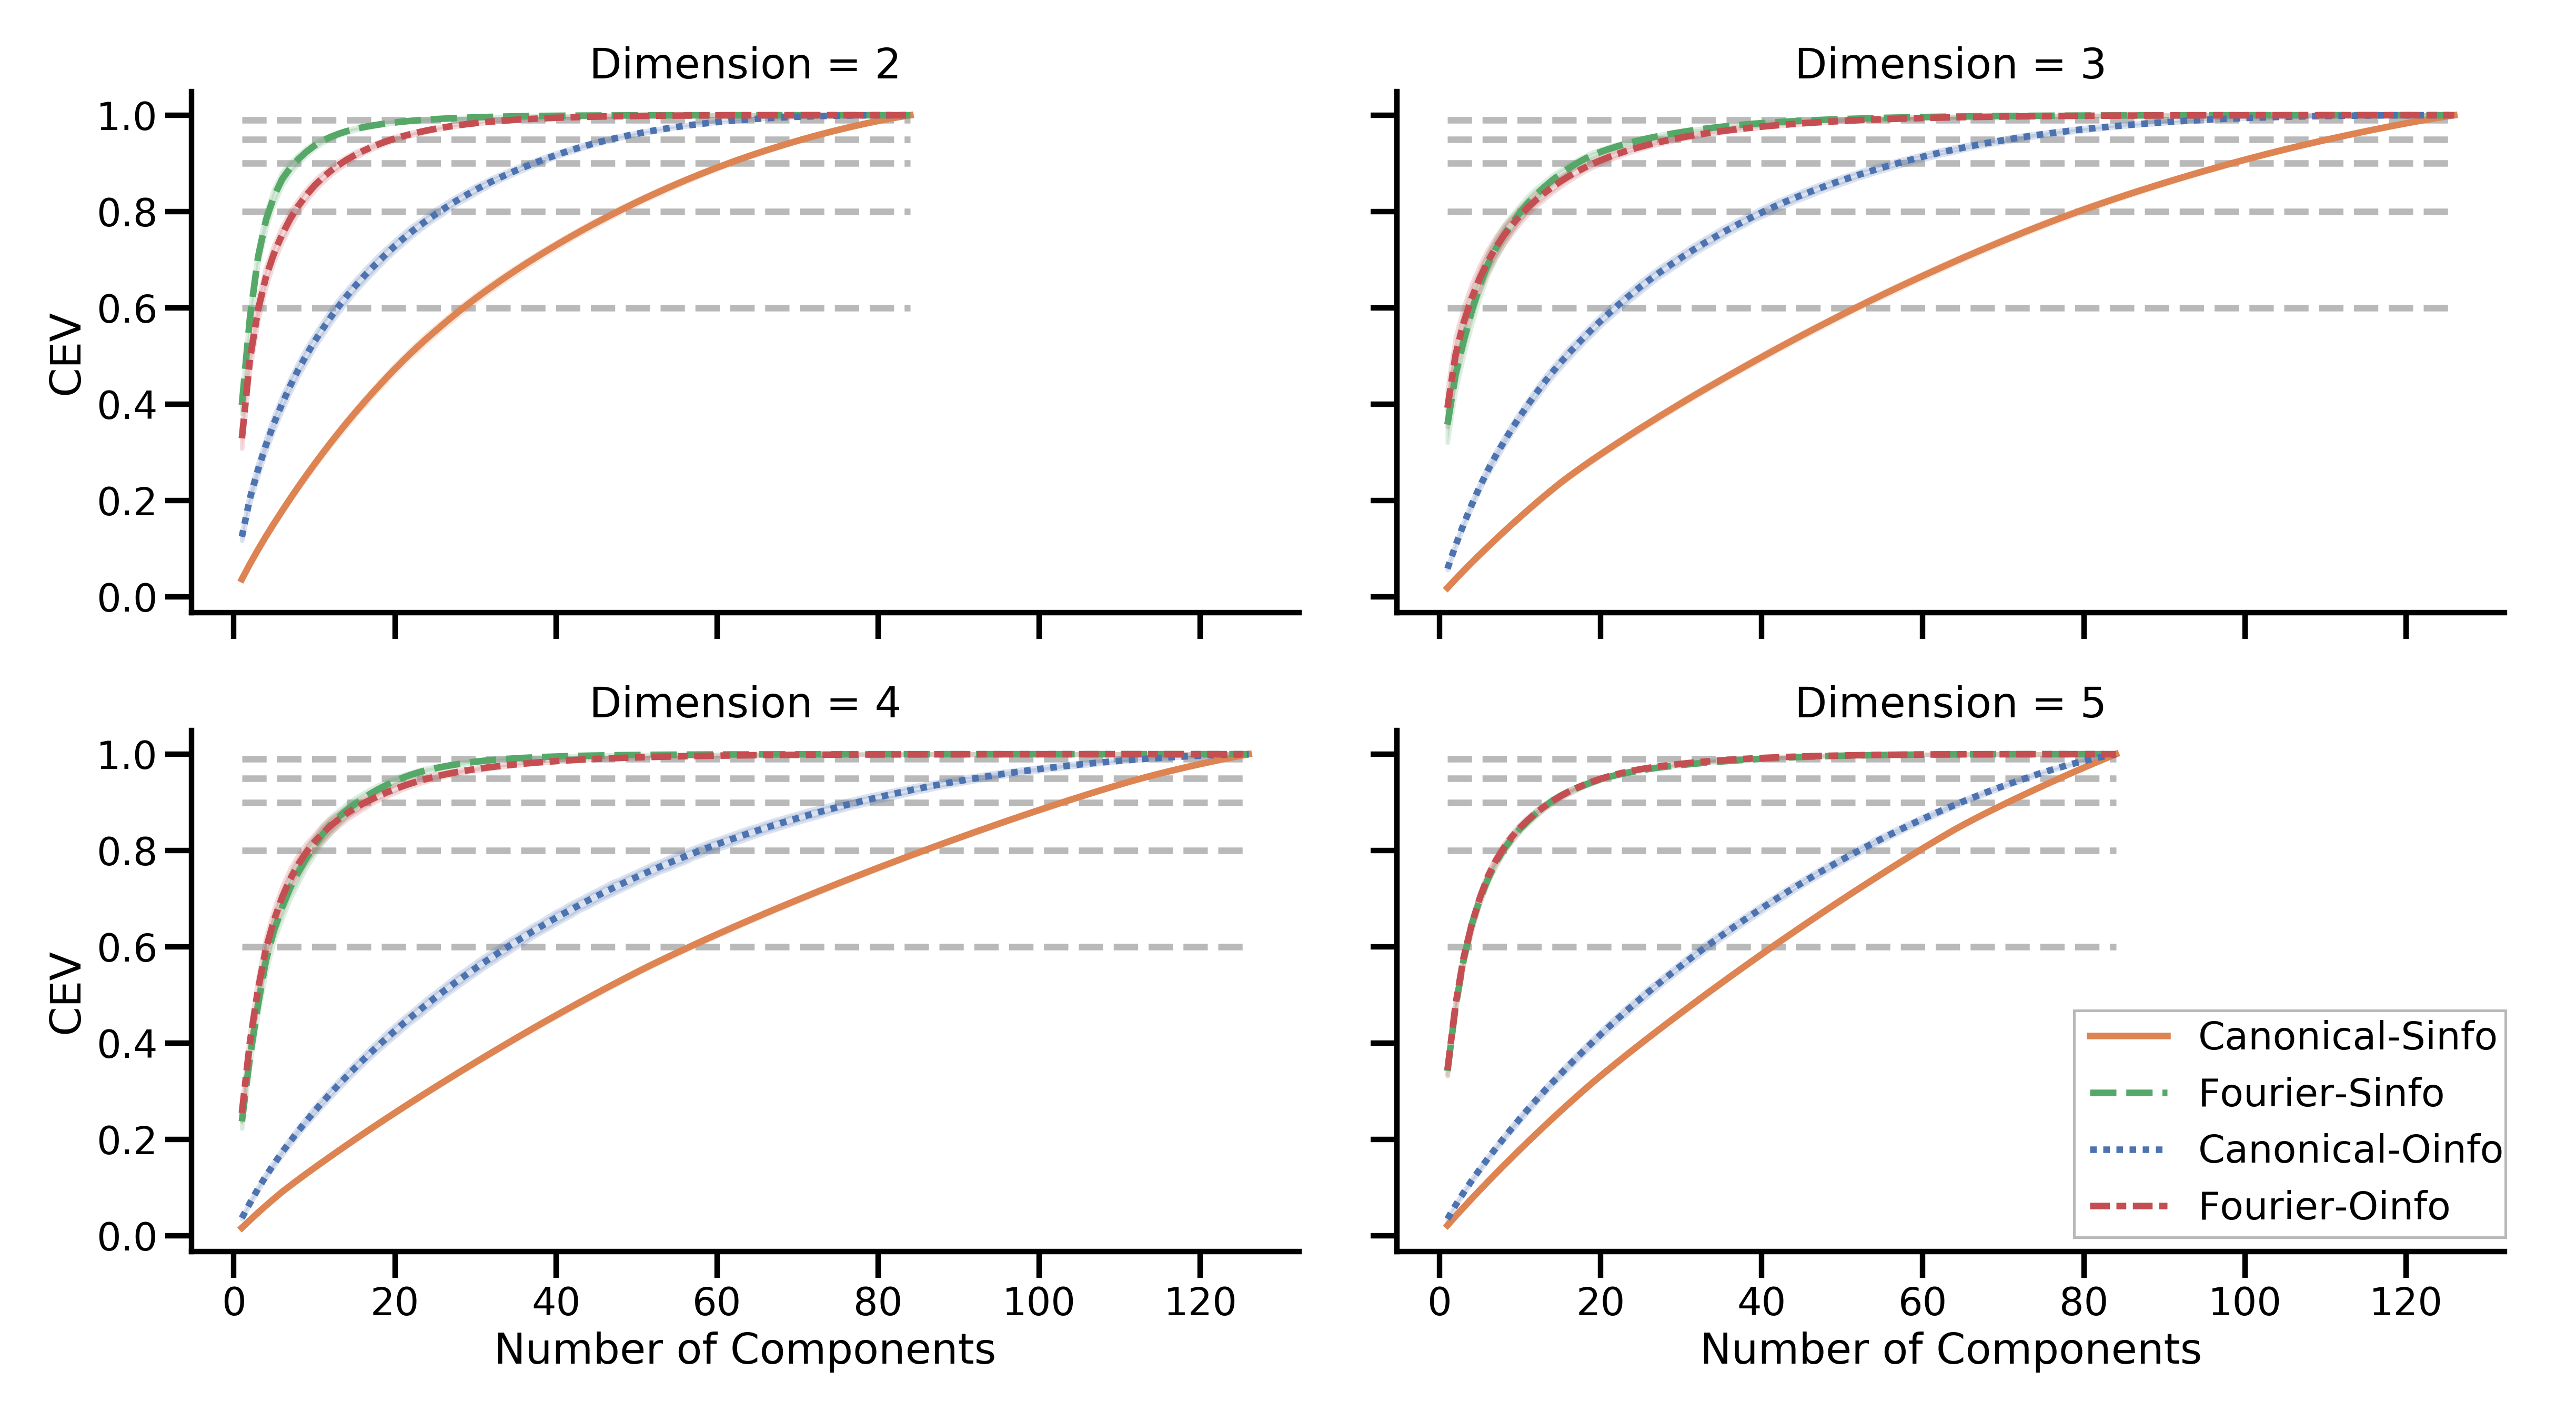
\includegraphics[scale=.092]{hyperharmonic}
\end{frame}

{
	\usebackgroundtemplate{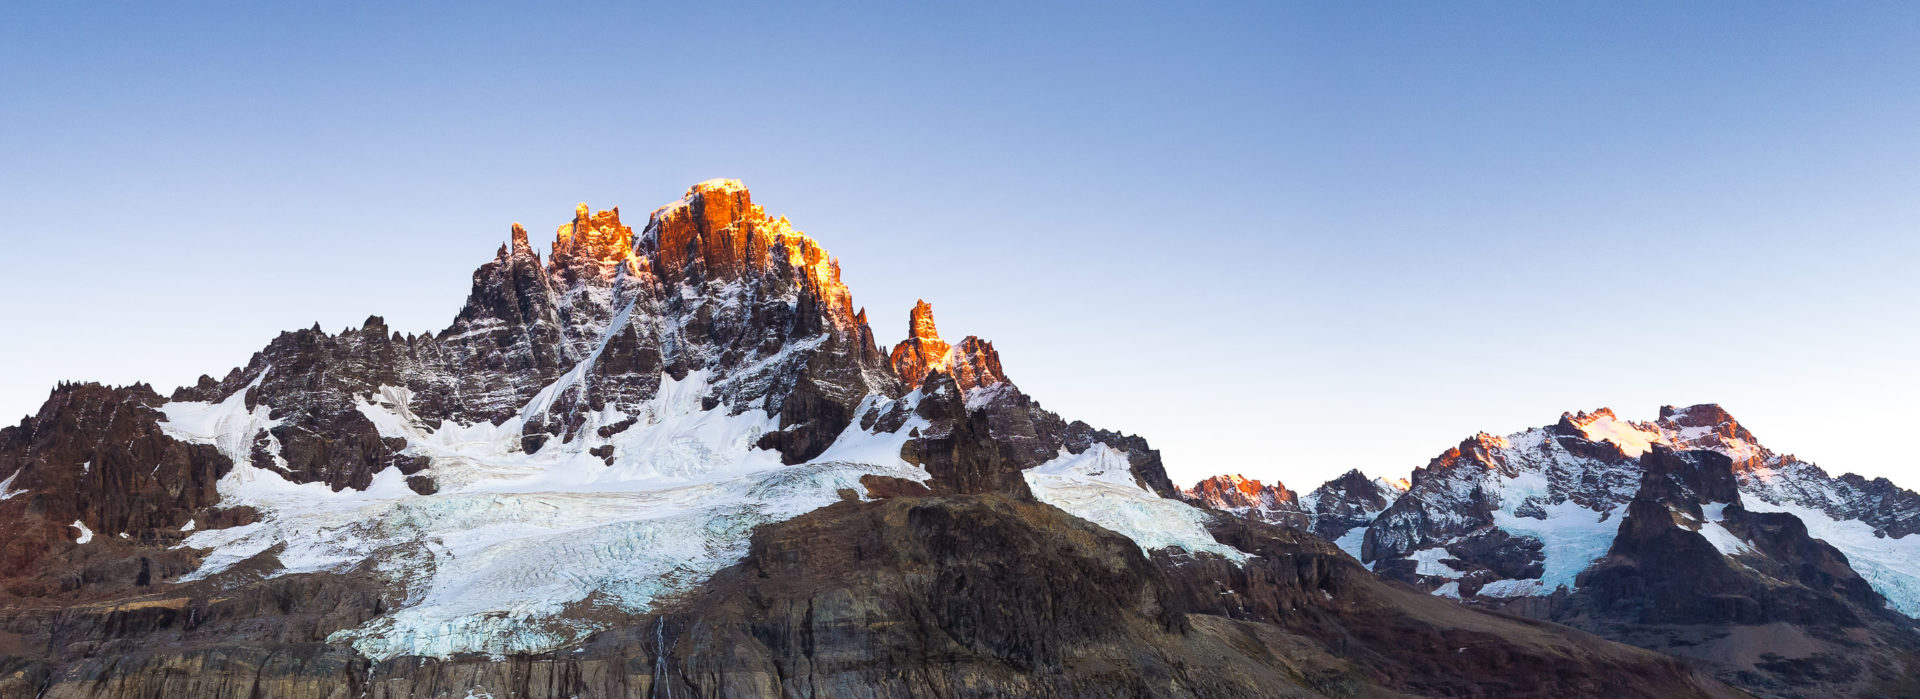
\includegraphics[width=\paperwidth]{castillo.jpg}}%
	\begin{frame}
		\vskip 6cm
		\begin{center}
			\textcolor{pblue}{\Huge Thank you}
		\end{center}
	\end{frame}
}


%\begin{frame}%[allowframebreaks]
%	\frametitle{Thank you!}
%	\nocite{whitney1935history}
%	\bibliographystyle{amsalpha}
%	\bibliography{biblio.bib}
%\end{frame}

\end{document}
